\section{Data} \label{data}

Regarding our data, we gathered scientific works from the WoS database from January 1, 1983 to December 31, 2024. We performed two searches in all editions of the Web of Science Core Collection, which provides the most complete bibliographic information that can be extracted from the WoS database and allows us to export every file in BibTex extension, which is one of the most recommended to handle bibliographic data. The first search gave us access to data with an excellent time span, while the second search was more extensive in terms of the keywords/terms considered and also gave us access to data of higher bibliographic quality.

Even though in the end the goal was to retrieve documents from the same field, the two searches were carried out using different strategies with the goal of complementing each other, thus forming the most complete and representative database. In the first search, we adopted a less restrictive search strategy, using a smaller set of keywords/terms and also being less strict regarding the quality of bibliographic information. This strategy led us to retrieve and add documents of lower bibliographic quality, that is, missing one or more elements from fields such as abstract or keywords, but that could still be useful. In the second search, we aimed at filling in the gaps left by the first search, retrieving and adding works that have been left out previously by using a broader list of keywords/terms, and adopting a search strategy that would retrieve only documents of the highest bibliographic quality, that is, works that contained almost all of the most important bibliographic elements, which is of the utmost importance for our topic modelling.

Unquestionably, the main concern during the data collection process was having at hand a dataset in which the documents belonged to the field of \textit{economics of migration}. In practical terms, to fulfil this condition, we had to make sure that (i) the documents belonged to the field of migration, and that (ii) those works were dealing with economic aspects of migration. In order to retrieve only documents on migration, we used a set of representative keywords/terms of migration studies in combination with different fields in the WoS advanced search tool\footnote{A file detailing how we conducted our searches in the WoS database, including all keywords and terms used, can be found in the data repository.}. After that, to keep only works dealing with economic aspects of migration, we applied filters in the Research Area and Web of Science Category fields in the WoS advanced search tool; specifically, we only considered scientific works that were simultaneously classified in the Research Area ``Business \& Economics" and in the Web of Science Category ``Economics", although not solely\footnote{Documents can belong to multiple Research Areas and Web of Science Categories. Here, we consider documents classified in those areas, solely or not, meaning that a document classified in multiple Research Areas and Web of Science Categories is suitable for us given that one of the Research Areas is ``Business \& Economics" and one of the Web of Science Categories is ``Economics". We think this is the right approach, considering that migration is multidisciplinary by nature, and has recently become more interdisciplinary, as shown in Appendix \ref{migration_studies}. Hence, if we had considered documents belonging only to the Research Area and Web of Science Category of interest, we would have been too strict, leaving out many documents that would fit our definition of \textit{economics of migration}.}.  Additional filters were applied in both searches to consider documents of all types but meeting abstracts, corrections, notes, letters, discussions, bibliographies, bibliographical-items, news items, reprints, and data papers\footnote{For a complete description of all document types available in the Web of Science Core Collection, see: \url{https://webofscience.help.clarivate.com/en-us/Content/document-types.html}.}, and documents written in English only.

Eventually, the first search retrieved 4,890 scientific works\footnote{This was the amount recorded the last time the search was performed before the database was exported. Attempted replications using the same settings may generate different results as the WoS databases are constantly being updated.}, out of which we added 4,696 to our dataset\footnote{The difference of the amount retrieved by the search and the amount added to our dataset, of 193 documents, is due to works that we decided to drop after individually reviewing and screening each document retrieved by the first search, a method applied to minimize the presence of off-topic documents.}. The second search retrieved 6,056 documents that were all added to the dataset. Summing up the two searches, we had a total of 10,752 documents, with 2,425 works common to both searches. After excluding the duplicates, we end up with the 8,327 documents. However, the WoS database do not include the abstracts of 971 of these documents, making them useless for our topic modelling strategy.

Thus, after removing the documents that did not have their abstracts included, we ended up with 7,386 scientific works from 1991 to 2024 (all the documents from 1983 to 1990 did not have their abstracts included), which constitute our final dataset. Below, we present some bibliographic information about our dataset, in order to show the main characteristics of the scientific research on the \textit{economics of migration}, such as scientific production, most frequent keywords, and most productive countries.

\subsection{Metadata} \label{metadata}

% the R package \textit{bibliometrix}\footnote{This R package provides the main tools to perform a bibliometric analysis. For a detailed presentation, see \cite{aria_bibliometrix_2017}.}

Regarding the document types, the vast majority are articles (both assigned to a final issue and early access) and proceedings papers. In addition, we have a total of 773 sources (journals, books, etc) and 11,131 different authors. Concerning the scientific production, Figure \ref{fig:annual_production} displays the quantity of scientific works published each year. As we can see, from 1991 until 2005, the production stayed below 100 documents per year, accelerating starting from 2006, and reaching a peak production of 671 documents in 2024.

\begin{figure}[!ht]
	\centering
	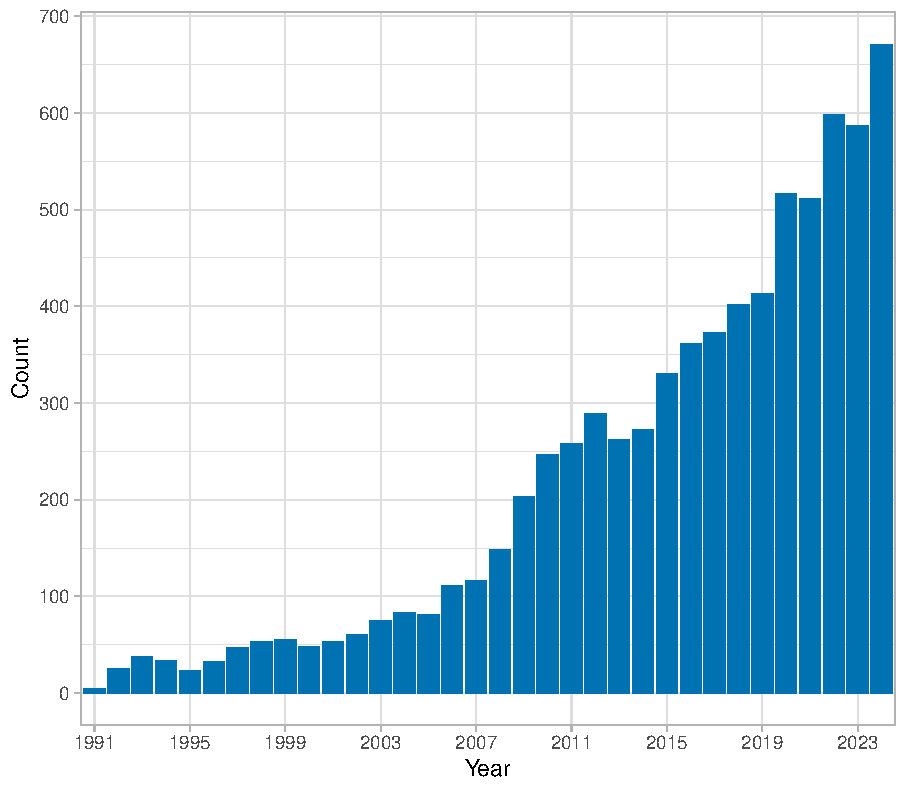
\includegraphics[width=0.75\linewidth]{annual_production.pdf}
	\caption{Yearly production of scientific works, 1991-2024.}
	\label{fig:annual_production}
\end{figure}

The twelve most relevant authors' keywords in our dataset, by the absolute number of occurrences, can be seen in Figure \ref{fig:most_relevant_AK}. The most frequent one was originally ``migration" with 1,686 appearances, but we decided to remove it because it does not add any semantic value to our analysis. For instance, if we intend to use the list of most relevant authors' keywords to gain an understanding of the topics that have been studied the most, the keyword ``migration" does not provide any useful information because it can refer to literally any topic we are dealing with. Also, in the list we have ``J61", which is the Journal of Economic Literature (JEL) code for ``Geographic Labor Mobility, Immigrant Workers". As we can see, the three most common words are directly related to international migration, with ``immigration" and ``remittances" ahead of the rest by a large margin. As a matter of fact, seven out of the twelve words are directly related to international migration: ``immigration", ``remittances", ``international migration", ``immigrants", ``refugees", ``J61", and ``brain drain". This may indicate a shift in the \textit{economics of migration} research, which, after focusing much more on internal migration throughout the last century, as seen in Section \ref{lit_review}, may now be turning its attention to international migration.

\begin{figure}[!ht]
	\centering
	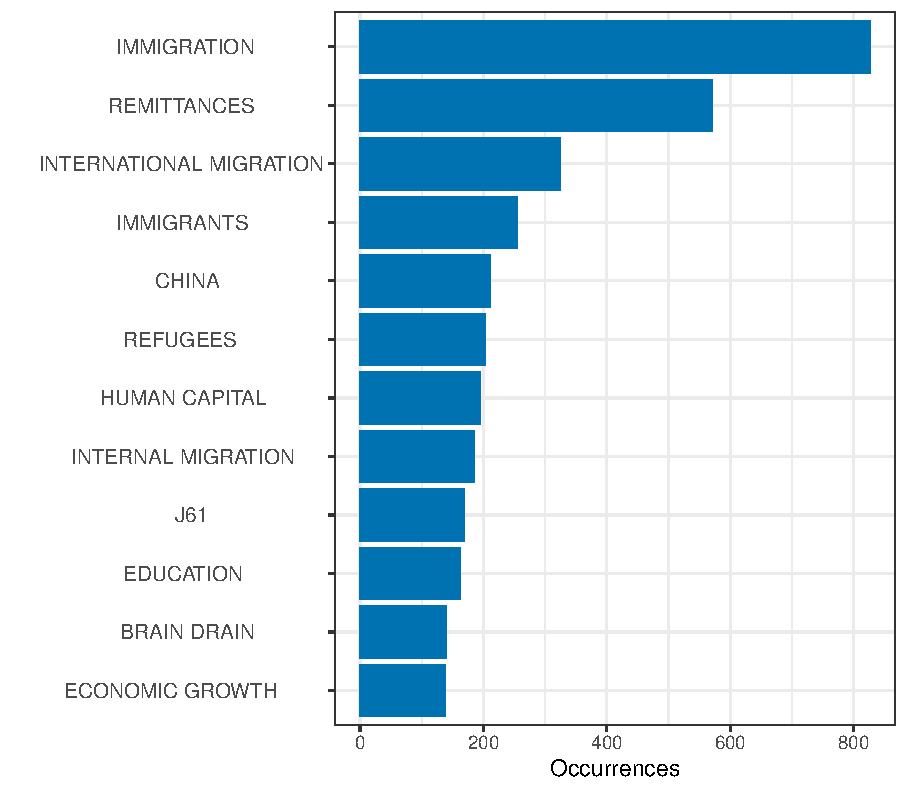
\includegraphics[width=0.75\textwidth]{most_relevant_AK_overall.pdf}
	\caption{The twelve most relevant authors' keywords in the whole dataset, by the absolute number of occurrences.}
	\label{fig:most_relevant_AK}
\end{figure}

Table \ref{tab:most_prod_countries} shows the ten most productive countries\footnote{To build Table \ref{tab:most_prod_countries}, we used one of the main bibliometric measures returned by the function \textit{biblioAnalysis} called \textit{Countries}, which according to \cite{aria_bibliometrix_2017}, it's the affiliation countries’ frequency distribution of all co-authors for each paper.} in terms of five metrics: number of documents, single country publications (SCP), multiple country publications (MCP), total number of citations, and average citation per document. From the figures shown, we highlight the United States, which leads in all metrics but the average document citation, where the United Kingdom is in the lead; and the relative low number of total citations in scientific papers linked to Chinese institutions, leading to a low average citation value per document. Overall, this table shows that research on the economics of migration is heavily concentrated in the United States, Canada, and Europe, aligning with what is seen in the field of migration studies, as shown in Appendix \ref{migration_studies}.


  \providecommand{\huxb}[2]{\arrayrulecolor[RGB]{#1}\global\arrayrulewidth=#2pt}
  \providecommand{\huxvb}[2]{\color[RGB]{#1}\vrule width #2pt}
  \providecommand{\huxtpad}[1]{\rule{0pt}{#1}}
  \providecommand{\huxbpad}[1]{\rule[-#1]{0pt}{#1}}

\begin{table}[ht]
\begin{centerbox}
\begin{threeparttable}
\setlength{\tabcolsep}{0pt}
\begin{tabular}{l l l l l l}


\hhline{>{\huxb{0, 0, 0}{0.4}}->{\huxb{0, 0, 0}{0.4}}->{\huxb{0, 0, 0}{0.4}}->{\huxb{0, 0, 0}{0.4}}->{\huxb{0, 0, 0}{0.4}}->{\huxb{0, 0, 0}{0.4}}-}
\arrayrulecolor{black}

\multicolumn{1}{!{\huxvb{0, 0, 0}{0}}c!{\huxvb{0, 0, 0}{0}}}{\huxtpad{6pt + 1em}\centering \hspace{6pt} \textbf{{\fontsize{6pt}{7.2pt}\selectfont Country}} \hspace{6pt}\huxbpad{6pt}} &
\multicolumn{1}{c!{\huxvb{0, 0, 0}{0}}}{\huxtpad{6pt + 1em}\centering \hspace{6pt} \textbf{{\fontsize{6pt}{7.2pt}\selectfont Number of Documents}} \hspace{6pt}\huxbpad{6pt}} &
\multicolumn{1}{c!{\huxvb{0, 0, 0}{0}}}{\huxtpad{6pt + 1em}\centering \hspace{6pt} \textbf{{\fontsize{6pt}{7.2pt}\selectfont SCP}} \hspace{6pt}\huxbpad{6pt}} &
\multicolumn{1}{c!{\huxvb{0, 0, 0}{0}}}{\huxtpad{6pt + 1em}\centering \hspace{6pt} \textbf{{\fontsize{6pt}{7.2pt}\selectfont MCP}} \hspace{6pt}\huxbpad{6pt}} &
\multicolumn{1}{c!{\huxvb{0, 0, 0}{0}}}{\huxtpad{6pt + 1em}\centering \hspace{6pt} \textbf{{\fontsize{6pt}{7.2pt}\selectfont Total citations}} \hspace{6pt}\huxbpad{6pt}} &
\multicolumn{1}{c!{\huxvb{0, 0, 0}{0}}}{\huxtpad{6pt + 1em}\centering \hspace{6pt} \textbf{{\fontsize{6pt}{7.2pt}\selectfont Average document citation}} \hspace{6pt}\huxbpad{6pt}} \tabularnewline[-0.5pt]


\hhline{>{\huxb{0, 0, 0}{0.4}}->{\huxb{0, 0, 0}{0.4}}->{\huxb{0, 0, 0}{0.4}}->{\huxb{0, 0, 0}{0.4}}->{\huxb{0, 0, 0}{0.4}}->{\huxb{0, 0, 0}{0.4}}-}
\arrayrulecolor{black}

\multicolumn{1}{!{\huxvb{0, 0, 0}{0}}c!{\huxvb{0, 0, 0}{0}}}{\huxtpad{6pt + 1em}\centering \hspace{6pt} {\fontsize{6pt}{7.2pt}\selectfont USA} \hspace{6pt}\huxbpad{6pt}} &
\multicolumn{1}{c!{\huxvb{0, 0, 0}{0}}}{\huxtpad{6pt + 1em}\centering \hspace{6pt} {\fontsize{6pt}{7.2pt}\selectfont 2,053} \hspace{6pt}\huxbpad{6pt}} &
\multicolumn{1}{c!{\huxvb{0, 0, 0}{0}}}{\huxtpad{6pt + 1em}\centering \hspace{6pt} {\fontsize{6pt}{7.2pt}\selectfont 1,563} \hspace{6pt}\huxbpad{6pt}} &
\multicolumn{1}{c!{\huxvb{0, 0, 0}{0}}}{\huxtpad{6pt + 1em}\centering \hspace{6pt} {\fontsize{6pt}{7.2pt}\selectfont 490} \hspace{6pt}\huxbpad{6pt}} &
\multicolumn{1}{c!{\huxvb{0, 0, 0}{0}}}{\huxtpad{6pt + 1em}\centering \hspace{6pt} {\fontsize{6pt}{7.2pt}\selectfont 67,826} \hspace{6pt}\huxbpad{6pt}} &
\multicolumn{1}{c!{\huxvb{0, 0, 0}{0}}}{\huxtpad{6pt + 1em}\centering \hspace{6pt} {\fontsize{6pt}{7.2pt}\selectfont 33.04} \hspace{6pt}\huxbpad{6pt}} \tabularnewline[-0.5pt]


\hhline{}
\arrayrulecolor{black}

\multicolumn{1}{!{\huxvb{0, 0, 0}{0}}c!{\huxvb{0, 0, 0}{0}}}{\huxtpad{6pt + 1em}\centering \hspace{6pt} {\fontsize{6pt}{7.2pt}\selectfont UNITED KINGDOM} \hspace{6pt}\huxbpad{6pt}} &
\multicolumn{1}{c!{\huxvb{0, 0, 0}{0}}}{\huxtpad{6pt + 1em}\centering \hspace{6pt} {\fontsize{6pt}{7.2pt}\selectfont 734} \hspace{6pt}\huxbpad{6pt}} &
\multicolumn{1}{c!{\huxvb{0, 0, 0}{0}}}{\huxtpad{6pt + 1em}\centering \hspace{6pt} {\fontsize{6pt}{7.2pt}\selectfont 458} \hspace{6pt}\huxbpad{6pt}} &
\multicolumn{1}{c!{\huxvb{0, 0, 0}{0}}}{\huxtpad{6pt + 1em}\centering \hspace{6pt} {\fontsize{6pt}{7.2pt}\selectfont 276} \hspace{6pt}\huxbpad{6pt}} &
\multicolumn{1}{c!{\huxvb{0, 0, 0}{0}}}{\huxtpad{6pt + 1em}\centering \hspace{6pt} {\fontsize{6pt}{7.2pt}\selectfont 25,252} \hspace{6pt}\huxbpad{6pt}} &
\multicolumn{1}{c!{\huxvb{0, 0, 0}{0}}}{\huxtpad{6pt + 1em}\centering \hspace{6pt} {\fontsize{6pt}{7.2pt}\selectfont 34.40} \hspace{6pt}\huxbpad{6pt}} \tabularnewline[-0.5pt]


\hhline{}
\arrayrulecolor{black}

\multicolumn{1}{!{\huxvb{0, 0, 0}{0}}c!{\huxvb{0, 0, 0}{0}}}{\huxtpad{6pt + 1em}\centering \hspace{6pt} {\fontsize{6pt}{7.2pt}\selectfont CHINA} \hspace{6pt}\huxbpad{6pt}} &
\multicolumn{1}{c!{\huxvb{0, 0, 0}{0}}}{\huxtpad{6pt + 1em}\centering \hspace{6pt} {\fontsize{6pt}{7.2pt}\selectfont 596} \hspace{6pt}\huxbpad{6pt}} &
\multicolumn{1}{c!{\huxvb{0, 0, 0}{0}}}{\huxtpad{6pt + 1em}\centering \hspace{6pt} {\fontsize{6pt}{7.2pt}\selectfont 416} \hspace{6pt}\huxbpad{6pt}} &
\multicolumn{1}{c!{\huxvb{0, 0, 0}{0}}}{\huxtpad{6pt + 1em}\centering \hspace{6pt} {\fontsize{6pt}{7.2pt}\selectfont 180} \hspace{6pt}\huxbpad{6pt}} &
\multicolumn{1}{c!{\huxvb{0, 0, 0}{0}}}{\huxtpad{6pt + 1em}\centering \hspace{6pt} {\fontsize{6pt}{7.2pt}\selectfont 9,422} \hspace{6pt}\huxbpad{6pt}} &
\multicolumn{1}{c!{\huxvb{0, 0, 0}{0}}}{\huxtpad{6pt + 1em}\centering \hspace{6pt} {\fontsize{6pt}{7.2pt}\selectfont 15.81} \hspace{6pt}\huxbpad{6pt}} \tabularnewline[-0.5pt]


\hhline{}
\arrayrulecolor{black}

\multicolumn{1}{!{\huxvb{0, 0, 0}{0}}c!{\huxvb{0, 0, 0}{0}}}{\huxtpad{6pt + 1em}\centering \hspace{6pt} {\fontsize{6pt}{7.2pt}\selectfont GERMANY} \hspace{6pt}\huxbpad{6pt}} &
\multicolumn{1}{c!{\huxvb{0, 0, 0}{0}}}{\huxtpad{6pt + 1em}\centering \hspace{6pt} {\fontsize{6pt}{7.2pt}\selectfont 516} \hspace{6pt}\huxbpad{6pt}} &
\multicolumn{1}{c!{\huxvb{0, 0, 0}{0}}}{\huxtpad{6pt + 1em}\centering \hspace{6pt} {\fontsize{6pt}{7.2pt}\selectfont 299} \hspace{6pt}\huxbpad{6pt}} &
\multicolumn{1}{c!{\huxvb{0, 0, 0}{0}}}{\huxtpad{6pt + 1em}\centering \hspace{6pt} {\fontsize{6pt}{7.2pt}\selectfont 217} \hspace{6pt}\huxbpad{6pt}} &
\multicolumn{1}{c!{\huxvb{0, 0, 0}{0}}}{\huxtpad{6pt + 1em}\centering \hspace{6pt} {\fontsize{6pt}{7.2pt}\selectfont 9,108} \hspace{6pt}\huxbpad{6pt}} &
\multicolumn{1}{c!{\huxvb{0, 0, 0}{0}}}{\huxtpad{6pt + 1em}\centering \hspace{6pt} {\fontsize{6pt}{7.2pt}\selectfont 17.65} \hspace{6pt}\huxbpad{6pt}} \tabularnewline[-0.5pt]


\hhline{}
\arrayrulecolor{black}

\multicolumn{1}{!{\huxvb{0, 0, 0}{0}}c!{\huxvb{0, 0, 0}{0}}}{\huxtpad{6pt + 1em}\centering \hspace{6pt} {\fontsize{6pt}{7.2pt}\selectfont ITALY} \hspace{6pt}\huxbpad{6pt}} &
\multicolumn{1}{c!{\huxvb{0, 0, 0}{0}}}{\huxtpad{6pt + 1em}\centering \hspace{6pt} {\fontsize{6pt}{7.2pt}\selectfont 365} \hspace{6pt}\huxbpad{6pt}} &
\multicolumn{1}{c!{\huxvb{0, 0, 0}{0}}}{\huxtpad{6pt + 1em}\centering \hspace{6pt} {\fontsize{6pt}{7.2pt}\selectfont 221} \hspace{6pt}\huxbpad{6pt}} &
\multicolumn{1}{c!{\huxvb{0, 0, 0}{0}}}{\huxtpad{6pt + 1em}\centering \hspace{6pt} {\fontsize{6pt}{7.2pt}\selectfont 144} \hspace{6pt}\huxbpad{6pt}} &
\multicolumn{1}{c!{\huxvb{0, 0, 0}{0}}}{\huxtpad{6pt + 1em}\centering \hspace{6pt} {\fontsize{6pt}{7.2pt}\selectfont 6,486} \hspace{6pt}\huxbpad{6pt}} &
\multicolumn{1}{c!{\huxvb{0, 0, 0}{0}}}{\huxtpad{6pt + 1em}\centering \hspace{6pt} {\fontsize{6pt}{7.2pt}\selectfont 17.77} \hspace{6pt}\huxbpad{6pt}} \tabularnewline[-0.5pt]


\hhline{}
\arrayrulecolor{black}

\multicolumn{1}{!{\huxvb{0, 0, 0}{0}}c!{\huxvb{0, 0, 0}{0}}}{\huxtpad{6pt + 1em}\centering \hspace{6pt} {\fontsize{6pt}{7.2pt}\selectfont CANADA} \hspace{6pt}\huxbpad{6pt}} &
\multicolumn{1}{c!{\huxvb{0, 0, 0}{0}}}{\huxtpad{6pt + 1em}\centering \hspace{6pt} {\fontsize{6pt}{7.2pt}\selectfont 312} \hspace{6pt}\huxbpad{6pt}} &
\multicolumn{1}{c!{\huxvb{0, 0, 0}{0}}}{\huxtpad{6pt + 1em}\centering \hspace{6pt} {\fontsize{6pt}{7.2pt}\selectfont 233} \hspace{6pt}\huxbpad{6pt}} &
\multicolumn{1}{c!{\huxvb{0, 0, 0}{0}}}{\huxtpad{6pt + 1em}\centering \hspace{6pt} {\fontsize{6pt}{7.2pt}\selectfont 79} \hspace{6pt}\huxbpad{6pt}} &
\multicolumn{1}{c!{\huxvb{0, 0, 0}{0}}}{\huxtpad{6pt + 1em}\centering \hspace{6pt} {\fontsize{6pt}{7.2pt}\selectfont 5,235} \hspace{6pt}\huxbpad{6pt}} &
\multicolumn{1}{c!{\huxvb{0, 0, 0}{0}}}{\huxtpad{6pt + 1em}\centering \hspace{6pt} {\fontsize{6pt}{7.2pt}\selectfont 16.78} \hspace{6pt}\huxbpad{6pt}} \tabularnewline[-0.5pt]


\hhline{}
\arrayrulecolor{black}

\multicolumn{1}{!{\huxvb{0, 0, 0}{0}}c!{\huxvb{0, 0, 0}{0}}}{\huxtpad{6pt + 1em}\centering \hspace{6pt} {\fontsize{6pt}{7.2pt}\selectfont AUSTRALIA} \hspace{6pt}\huxbpad{6pt}} &
\multicolumn{1}{c!{\huxvb{0, 0, 0}{0}}}{\huxtpad{6pt + 1em}\centering \hspace{6pt} {\fontsize{6pt}{7.2pt}\selectfont 266} \hspace{6pt}\huxbpad{6pt}} &
\multicolumn{1}{c!{\huxvb{0, 0, 0}{0}}}{\huxtpad{6pt + 1em}\centering \hspace{6pt} {\fontsize{6pt}{7.2pt}\selectfont 173} \hspace{6pt}\huxbpad{6pt}} &
\multicolumn{1}{c!{\huxvb{0, 0, 0}{0}}}{\huxtpad{6pt + 1em}\centering \hspace{6pt} {\fontsize{6pt}{7.2pt}\selectfont 93} \hspace{6pt}\huxbpad{6pt}} &
\multicolumn{1}{c!{\huxvb{0, 0, 0}{0}}}{\huxtpad{6pt + 1em}\centering \hspace{6pt} {\fontsize{6pt}{7.2pt}\selectfont 5,737} \hspace{6pt}\huxbpad{6pt}} &
\multicolumn{1}{c!{\huxvb{0, 0, 0}{0}}}{\huxtpad{6pt + 1em}\centering \hspace{6pt} {\fontsize{6pt}{7.2pt}\selectfont 21.57} \hspace{6pt}\huxbpad{6pt}} \tabularnewline[-0.5pt]


\hhline{}
\arrayrulecolor{black}

\multicolumn{1}{!{\huxvb{0, 0, 0}{0}}c!{\huxvb{0, 0, 0}{0}}}{\huxtpad{6pt + 1em}\centering \hspace{6pt} {\fontsize{6pt}{7.2pt}\selectfont FRANCE} \hspace{6pt}\huxbpad{6pt}} &
\multicolumn{1}{c!{\huxvb{0, 0, 0}{0}}}{\huxtpad{6pt + 1em}\centering \hspace{6pt} {\fontsize{6pt}{7.2pt}\selectfont 252} \hspace{6pt}\huxbpad{6pt}} &
\multicolumn{1}{c!{\huxvb{0, 0, 0}{0}}}{\huxtpad{6pt + 1em}\centering \hspace{6pt} {\fontsize{6pt}{7.2pt}\selectfont 149} \hspace{6pt}\huxbpad{6pt}} &
\multicolumn{1}{c!{\huxvb{0, 0, 0}{0}}}{\huxtpad{6pt + 1em}\centering \hspace{6pt} {\fontsize{6pt}{7.2pt}\selectfont 103} \hspace{6pt}\huxbpad{6pt}} &
\multicolumn{1}{c!{\huxvb{0, 0, 0}{0}}}{\huxtpad{6pt + 1em}\centering \hspace{6pt} {\fontsize{6pt}{7.2pt}\selectfont 6,317} \hspace{6pt}\huxbpad{6pt}} &
\multicolumn{1}{c!{\huxvb{0, 0, 0}{0}}}{\huxtpad{6pt + 1em}\centering \hspace{6pt} {\fontsize{6pt}{7.2pt}\selectfont 25.07} \hspace{6pt}\huxbpad{6pt}} \tabularnewline[-0.5pt]


\hhline{}
\arrayrulecolor{black}

\multicolumn{1}{!{\huxvb{0, 0, 0}{0}}c!{\huxvb{0, 0, 0}{0}}}{\huxtpad{6pt + 1em}\centering \hspace{6pt} {\fontsize{6pt}{7.2pt}\selectfont SPAIN} \hspace{6pt}\huxbpad{6pt}} &
\multicolumn{1}{c!{\huxvb{0, 0, 0}{0}}}{\huxtpad{6pt + 1em}\centering \hspace{6pt} {\fontsize{6pt}{7.2pt}\selectfont 240} \hspace{6pt}\huxbpad{6pt}} &
\multicolumn{1}{c!{\huxvb{0, 0, 0}{0}}}{\huxtpad{6pt + 1em}\centering \hspace{6pt} {\fontsize{6pt}{7.2pt}\selectfont 173} \hspace{6pt}\huxbpad{6pt}} &
\multicolumn{1}{c!{\huxvb{0, 0, 0}{0}}}{\huxtpad{6pt + 1em}\centering \hspace{6pt} {\fontsize{6pt}{7.2pt}\selectfont 67} \hspace{6pt}\huxbpad{6pt}} &
\multicolumn{1}{c!{\huxvb{0, 0, 0}{0}}}{\huxtpad{6pt + 1em}\centering \hspace{6pt} {\fontsize{6pt}{7.2pt}\selectfont 3,984} \hspace{6pt}\huxbpad{6pt}} &
\multicolumn{1}{c!{\huxvb{0, 0, 0}{0}}}{\huxtpad{6pt + 1em}\centering \hspace{6pt} {\fontsize{6pt}{7.2pt}\selectfont 16.60} \hspace{6pt}\huxbpad{6pt}} \tabularnewline[-0.5pt]


\hhline{}
\arrayrulecolor{black}

\multicolumn{1}{!{\huxvb{0, 0, 0}{0}}c!{\huxvb{0, 0, 0}{0}}}{\huxtpad{6pt + 1em}\centering \hspace{6pt} {\fontsize{6pt}{7.2pt}\selectfont NETHERLANDS} \hspace{6pt}\huxbpad{6pt}} &
\multicolumn{1}{c!{\huxvb{0, 0, 0}{0}}}{\huxtpad{6pt + 1em}\centering \hspace{6pt} {\fontsize{6pt}{7.2pt}\selectfont 194} \hspace{6pt}\huxbpad{6pt}} &
\multicolumn{1}{c!{\huxvb{0, 0, 0}{0}}}{\huxtpad{6pt + 1em}\centering \hspace{6pt} {\fontsize{6pt}{7.2pt}\selectfont 127} \hspace{6pt}\huxbpad{6pt}} &
\multicolumn{1}{c!{\huxvb{0, 0, 0}{0}}}{\huxtpad{6pt + 1em}\centering \hspace{6pt} {\fontsize{6pt}{7.2pt}\selectfont 67} \hspace{6pt}\huxbpad{6pt}} &
\multicolumn{1}{c!{\huxvb{0, 0, 0}{0}}}{\huxtpad{6pt + 1em}\centering \hspace{6pt} {\fontsize{6pt}{7.2pt}\selectfont 4,092} \hspace{6pt}\huxbpad{6pt}} &
\multicolumn{1}{c!{\huxvb{0, 0, 0}{0}}}{\huxtpad{6pt + 1em}\centering \hspace{6pt} {\fontsize{6pt}{7.2pt}\selectfont 21.09} \hspace{6pt}\huxbpad{6pt}} \tabularnewline[-0.5pt]


\hhline{>{\huxb{0, 0, 0}{0.4}}->{\huxb{0, 0, 0}{0.4}}->{\huxb{0, 0, 0}{0.4}}->{\huxb{0, 0, 0}{0.4}}->{\huxb{0, 0, 0}{0.4}}->{\huxb{0, 0, 0}{0.4}}-}
\arrayrulecolor{black}
\end{tabular}\captionsetup{justification=centering,singlelinecheck=off}
\caption{The ten most productive countries in terms of total number of documents published, collaboration indices SCP and MCP, total number of citations, and average citation per document, 1991-2024.}
 \label{tab:most_prod_countries}

\end{threeparttable}\par\end{centerbox}

\end{table}
